\section{External Interface Requirements}
\label{sec:external_interface_requirements}%

\subsection{User Interfaces}
\label{subsec:user_interfaces}%
The eMALL’s user interfaces are a website and a mobile application;
the first is developed to be used mainly by CPOs with a dedicated login section for businesses but can be used by EVDs too.
The mobile application is available for Android and iOS and provides an enhanced experience as compared to the website
since it offers users personalized suggestions based on their location.
The website and the app should be easy to use since they will be used mostly by middle-aged users,
who might not always be familiar with the technology.
A “quick booking” section dedicated to facilitating the booking process might be included,
for those EVDs who are used to booking a charge at the same charging station (based on suggestions given by AI).

\subsection{Hardware Interfaces}
\label{subsec:hardware_interfaces}%
The system only requires a smartphone or computer with an internet connection and web browser to access websites or mobile applications.
Furthermore, eMALL communicates with the EV through its company's API to get the current battery level, the charging state,
so if it is plugged in and if it is charging, and the number of routable kilometers obtained on the current battery level.
To access personalized suggestions, based on EV’s position, the device in use has to be able to detect its location with a GPS or Glonass localization system.

\subsection{Software Interfaces}
\label{subsec:software_interfaces}%
%TODO: complete the section
The following list describes the required software interfaces that the \verb|eMALL| system uses:
\begin{itemize}
    \item \textbf{CPMS and Charging Points.} The CPMS that is offered to the CPO communicates with the charging points
    through their API\@.
    Thanks to it, the system can manage the charging session, given the possibility of starting and stopping it.
    Another significant functionality is the diagnostic of the charging point:
    a CPO can reboot its charging spots, can get their log, and can update their firmware.
    %TODO: Does it make sense to put an example of an external system
    \item \textbf{eMALL and EVs.} The eMALL system communicates with the EVs registered by the EVD\@.
    As explained in the domain assumption section, we suppose that there is a third-party system that offers its API
    so to get the status of the battery of the EV\@.
    %An example of a system that provides these features is Smartcar,
    %which is already used by companies like AmpUp or BeCharge to remotely retrieve the battery level and remaining range of the EVs.
    \item \textbf{CPMS and DSOs.} The CPMSs offered to the CPO communicate with the DSOs through their APIs.
    CPOs can get selling prices set by the DSOs and they can decide from which DSO to acquire electricity.
    \item \textbf{eMALL and third-party payment services.} The \verb|eMALL| system offers the possibility to pay through
    external payment services to the EVD. The communication happens thanks to APIs offered by the companies that handle payments.
\end{itemize}

\subsection{Communication Interfaces}
\label{subsec:communication_interfaces}%
%TODO: explain why TCP/IP is the best communication protocol for the eMALL system
%TODO: identify interfaces (OCPP and others)
The communication protocols that the \verb|eMALL| system uses are:
\begin{itemize}
    \item \textbf{Open Charge Point Protocol (OCPP).} It is used for the communication between the CPMS and the charging
    stations.
    \item \textbf{HTTP(S).} It is used when external APIs are exploited to retrieve data through the web, such as
    the communication between the \verb|eMALL| system and the DSOs and third-party payment services.
\end{itemize}


\section{Functional Requirements}
\label{sec:functional_requirements}%

\subsection{Requirements}
\label{subsec: requirements}%
\newcounter{req}
\setcounter{req}{1}
\newcommand{\creq}{\thereq\stepcounter{req}}
\begin{center}
%TODO: complete the table after having completed the use cases
    \begin{longtable}{|l|l|}
        \hline
        \textbf{ID} & \textbf{Description} \\
        \hline
        R\creq      &                      \\
        \hline
        \caption{Requirements.}
        \label{tab: req}%
    \end{longtable}
\end{center}

\subsection{Mapping on goals}
\label{subsec: map_on_g}%
\newcounter{mg}
\setcounter{mg}{1}
\newcommand{\cmg}{\themg\stepcounter{mg}}
\begin{center}
%TODO: complete the table after having done the requirements
    \begin{longtable}{|l|l|l|}
        \hline
        \textbf{Goal} & \textbf{Domain assumptions} & \textbf{Requirements} \\
        \hline
        G\cmg         &                             &                       \\
        \hline
        G\cmg         &                             &                       \\
        \hline
        G\cmg         &                             &                       \\
        \hline
        G\cmg         &                             &                       \\
        \hline
        G\cmg         &                             &                       \\
        \hline
        G\cmg         &                             &                       \\
        \hline
        G\cmg         &                             &                       \\
        \hline
        G\cmg         &                             &                       \\
        \hline
        G\cmg         &                             &                       \\
        \hline
        G\cmg         &                             &                       \\
        \hline
        G\cmg         &                             &                       \\
        \hline
        G\cmg         &                             &                       \\
        \hline
        \caption{Mapping on goals.}
        \label{tab: map_on_g}%
    \end{longtable}
\end{center}

\subsection{Use case diagrams}
\label{subsec: use_case_diag}%
%TODO: correct the diagrams if you add or remove use cases
\textbf{Unregistered EVD}
\begin{figure} [H]
    \begin{center}
        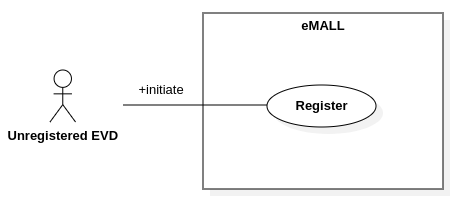
\includegraphics[width=0.9\linewidth]{Images/UseCaseDiagrams/unregistered_EVD_use_case_diagram}
        \caption{Unregistered EVD use case diagram}
        \label{fig: unreg_EVD_diag}
    \end{center}
\end{figure}

\textbf{Registered EVD}
\begin{figure} [H]
    \begin{center}
        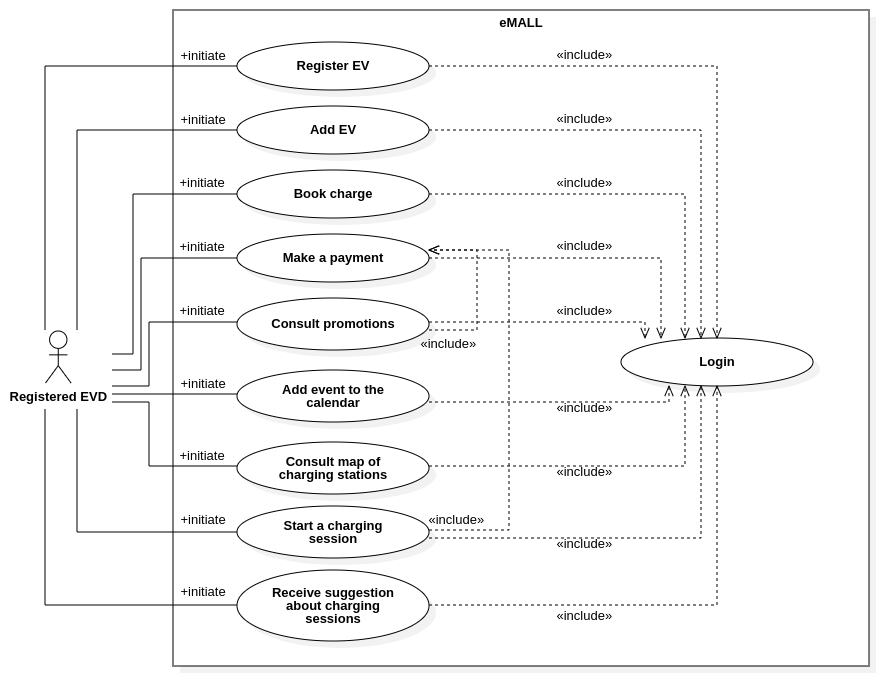
\includegraphics[width=0.9\linewidth]{Images/UseCaseDiagrams/registered_EVD_use_case_diagram}
        \caption{Unregistered EVD use case diagram}
        \label{fig: reg_EVD_diag}
    \end{center}
\end{figure}

\textbf{CPO}
\begin{figure} [H]
    \begin{center}
        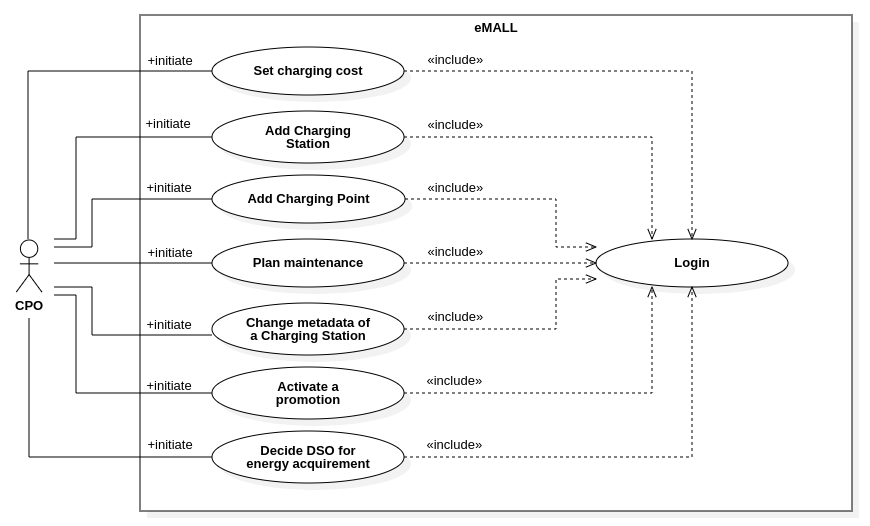
\includegraphics[width=0.9\linewidth]{Images/UseCaseDiagrams/CPO_use_case_diagram}
        \caption{Unregistered EVD use case diagram}
        \label{fig: cpo_diag}
    \end{center}
\end{figure}

\subsection{Use cases}
\label{subsec: use_cases}%
%TODO: write it better
In this section, they are explained and represented the main identified use cases.
There is a table with entry conditions, event flow, exit conditions and exception for each of them, and a sequence diagram
that shows the messages exchanged between the entities and the called functions. \\
%TODO: find new use cases
%TODO: insert sequence diagrams
%TODO: insert exeptions
\textbf{EVD registration.}
\begin{center}
    \begin{longtable}{lp{0.75\linewidth}}
        \hline
        Actor            & Unregistered EVD                                                                                                                                                                                      \\
        \hline
        Entry conditions & The EVD isn’t registered in the eMALL system, and he clicks the sign-up button                                                                                                                        \\
        \hline
        Event Flow       & 1. eMALL asks the unregistered EVD to insert personal information (i.e., name, surname, birthday, billing address, e-mail, and password).                                                             \\
        & 2. The unregistered EVD fills out the form with his personal information (name, surname, birthday, billing address, e-mail, and password) and accepts the “Terms \& Conditions” and “Privacy Policy”. \\
        & 3. eMALL validates the inserted EVD’s personal information.                                                                                                                                           \\
        & 4. eMALL asks the unregistered EVD to insert payment method information.                                                                                                                              \\
        & 5. The EVD fills out a form with its payment method information.                                                                                                                                      \\
        & 6. eMALL validates the inserted EVD’s payment method.                                                                                                                                                 \\
        & 7. eMALL sends a confirmation email to the EVD.                                                                                                                                                       \\
        & 8. eMALL sends back the EVD’s registration outcome.                                                                                                                                                   \\
        \hline
        Exit condition   & An account is created.                                                                                                                                                                                \\
        \hline
        Exceptions       & 3.1. eMALL isn’t able to validate the EVD’s personal information.                                                                                                                                     \\
        & 6.1. eMALL isn’t able to validate the EVD’s payment method.                                                                                                                                           \\
        & In all these cases, the user is notified with an error message.                                                                                                                                       \\
        \hline
        \caption{EVD registration use case.}
        \label{tab: EVD_sign_up_use_case}
    \end{longtable}
\end{center}

\textbf{EVD logs in.}
\begin{center}
    \begin{longtable}{lp{0.75\linewidth}}
        \hline
        Actor            & Registered EVD                                                                                                    \\
        \hline
        Entry conditions & The EVD is registered in the eMALL system and he clicks the log in button.                                        \\
        \hline
        Event Flow       & 1. eMALL asks the registered EVD to insert the e-mail.                                                            \\
        & 2. The registered EVD inserts the e-mail.                                                                         \\
        & 3. eMALL validates the inserted e-mail.                                                                           \\
        & 4. eMALL asks the registered EVD to insert the password associated with the e-mail.                               \\
        & 5. The registered EVD inserts the password.                                                                       \\
        & 6. eMALL validates the inserted password in combination with the e-mail.                                          \\
        & 7. eMALL sends back the login outcome.                                                                            \\
        \hline
        Exit condition   & The EVD access the eMALL system.                                                                                  \\
        \hline
        Exceptions       & 3.1 The e-mail is not recognized.                                                                                 \\
        & 6.1 The password is not correct.                                                                                  \\
        & In both cases, the user receives a notification through an error message. He has to insert his credentials again. \\
        \hline
        \caption{EVD logs in use case.}
        \label{tab: EVD_logs_in_use_case}
    \end{longtable}
\end{center}

\textbf{EVD adds an EV.}
\begin{center}
    \begin{longtable}{lp{0.75\linewidth}}
        \hline
        Actor            & Registered EVD                                                                                \\
        \hline
        Entry conditions & The EVD is registered and correctly logged in.                                                \\
        & The EVD clicks the ``Add a Vehicle'' button from his profile section of eMALL                 \\
        \hline
        Event Flow       & 1. eMALL asks the registered EVD to insert car informations.                                  \\
        & 2. The registered EVD inserts the requested information and he sends them to the eMALL.       \\
        & 3. eMALL validates the information searching for possible errors.                             \\
        & 4. eMALL asks the registered EVD to insert a nickname for the vehicle to save in his profile. \\
        & 5. The registered EVD inserts the nickame.                                                    \\
        & 6. eMALL validates the nickname also searching for duplicates between user EV nicknames.      \\
        & 7. eMALL sends back the registration outcome.                                                 \\
        \hline
        Exit condition   & EVD car information are not coherent or correct.                                              \\
        \hline
        Exceptions       & 3.1 The e-mail is not recognized.                                                             \\
        & 5.1 The inserted nickname is already taken between those owned by the user.                   \\
        & In both cases, the user receives a notification through an error message.                     \\
        \hline
        \caption{EVD adds an EV use case.}
        \label{tab: EVD_adds_a_vehicle_use_case}
    \end{longtable}
\end{center}

\textbf{Registered EVD books a charge.}
\begin{center}
    \begin{longtable}{lp{0.75\linewidth}}
        \hline
        Actor            & Registered EVD                                                                             \\
        \hline
        Entry conditions & The EVD is registered and correctly logged in.                                             \\
        & The EVD selects a specific charging station and clicks the ``book'' button                 \\
        \hline
        Event Flow       & 1. eMALL asks the registered EVD to choose a timeframe.                                    \\
        & 2. The registered EVD inserts the timeframe.                                               \\
        & 3. eMALL checks if the selected timeframe is currently available.                          \\
        & 4. eMALL selects a charging point to reserve for the EVD depending on EV's specifications. \\
        & 5. eMALL asks the registered EVD to confirm the booking with the prompted information.     \\
        & 6. The registered EVD clicks the ``Confir'' button to confirm the booking.                 \\
        & 7. eMALL adds the booking to the EVD's calendar.                                           \\
        & 8. eMALL sends back the booking outcome.                                                   \\
        \hline
        Exit condition   & A charging session is booked.                                                              \\
        \hline
        Exceptions       & 3.1. No free charging points are available at the selected timeframe.                      \\
        & The user is notified with an error message, and asked to select a new timeframe.           \\
        \hline
        \caption{EVD books a charge use case.}
        \label{tab: EVD_booking_use_case}
    \end{longtable}
\end{center}

\textbf{EVD consults the map of charging stations.}
\begin{center}
    \begin{longtable}{lp{0.75\linewidth}}
        \hline
        Actor            & Registered EVD                                                                                     \\
        \hline
        Entry conditions & The EVD is registered and correctly logged in.                                                     \\
        & The EVD is in the map section at a given or specified location.                                    \\
        \hline
        Event Flow       & 1. eMALL shows the map with all the charging stations available over a specific location.          \\
        & 2. The registered EVD moves on the map, searching for a charging station.                          \\
        & 3. eMALL retrieves the charging station locations in the new place.                                \\
        & 4. The registered EVD selects a specific charging station to get its detailed information.         \\
        & 5. eMALL retrieves the charging station's detailed information.                                    \\
        \hline
        Exit condition   & The registered EVD changes section, and moves from the dashboard.                                  \\
        \hline
        Exceptions       & 1.1 The user didn’t accept sharing location.                                                       \\
        & In this case, the user is notified by an error message and needs to move to its position manually. \\
        \hline
        \caption{EVD consults the map of charging stations use case.}
        \label{tab: EVD_map_charging_stations_use_case}
    \end{longtable}
\end{center}

\textbf{Registered EVD consults a specific promotion that can be redeemed.}
\begin{center}
    \begin{longtable}{lp{0.75\linewidth}}
        \hline
        Actor            & Registered EVD                                                                                                        \\
        \hline
        Entry conditions & The EVD is registered and correctly logged in.                                                                        \\
        & The EVD is in the promotion section.                                                                                  \\
        \hline
        Event Flow       & 1. eMALL sends the promotion list to the registered EVD.                                                              \\
        & 2. The registered EVD selects a promotion to activate.                                                                \\
        & 3. The registered EVD triggers the offer.                                                                             \\
        & 4. eMALL asks the registered EVD to choose between his payment methods.                                               \\
        & 5. The registered EVD picks the payment method.                                                                       \\
        & 6. eMALL asks the registered EVD to confirm the payment.                                                              \\
        & 7. The registered EVD authorizes the payment.                                                                         \\
        & 8. eMALL makes the payment.                                                                                           \\
        & 9. eMALL sends back the payment outcome.                                                                              \\
        \hline
        Exit condition   & The promotion has been activated.                                                                                     \\
        \hline
        Exceptions       & 8.1. The payment fails due to no sufficient funds.                                                                    \\
        & 8.2. The payment fails due to the failure of the transaction.                                                         \\
        & 8.3. The payment fails because of data input errors.                                                                   \\
        & 8.4. The payment fails due to technical issues.                                                                       \\
        & In these cases, the registered EVD receives a notification with an error message, and the promotion is not activated. \\
        \hline
        \caption{EVD consults a specific promotion that can be redeemed use case.}
        \label{tab: EVD_consults_promotion_use_case}
    \end{longtable}
\end{center}

\textbf{Registered EVD adds a new event to the calendar.}
\begin{center}
    \begin{longtable}{lp{0.75\linewidth}}
        \hline
        Actor            & Registered EVD                                                                                     \\
        \hline
        Entry conditions & The EVD is registered and correctly logged in.                                                     \\
        & The EVD is in the map section.                                                                     \\
        \hline
        Event Flow       & 1. eMALL shows the map with all the charging stations available over a specific location.          \\
        & 2. The registered EVD moves on the map, searching for a charging station.                          \\
        & 3. eMALL retrieves the charging station locations in the new place.                                \\
        & 4. The registered EVD selects a specific charging station to get its detailed information.         \\
        & 5. eMALL retrieves the charging station's detailed information.                                    \\
        \hline
        Exit condition   & The registered EVD changes section, and moves from the dashboard.                                  \\
        \hline
        Exceptions       & 1.1 The user didn’t accept sharing location.                                                       \\
        & In this case, the user is notified by an error message and needs to move to its position manually. \\
        \hline
        \caption{EVD adds a new event to the calendar use case.}
        \label{tab: EVD_adds_event_use_case}
    \end{longtable}
\end{center}

\textbf{CPO logs in.}
\begin{center}
    \begin{longtable}{lp{0.75\linewidth}}
        \hline
        Actor            & CPO                                                                                                 \\
        \hline
        Entry conditions & CPO’s operator is in the business login section.                                                    \\
        \hline
        Event Flow       & 1. eMALL asks the CPO operator to insert his credentials to log in.                                 \\
        & 2. The CPO operator inserts the CPO ID associated with its company, password, and email.            \\
        & 3. eMALL validates the inserted credentials combination.                                            \\
        & 4. eMALL sends back the login outcome.                                                              \\
        \hline
        Exit condition   & The CPO access the business section of the eMALL system                                             \\
        \hline
        Exceptions       & 3.1.1. CPO credentials are not correct and not validated by eMALL.                                  \\
        & 3.2.1. CPO’s affiliate agreement has expired, and its ID is no longer allowed to access the system. \\
        & In both cases, the user receives a notification with an error message.                              \\
        & Also, in the second case, the operator is invited to call the sales team.                           \\
        \hline
        \caption{CPO logs in use case.}
        \label{tab: CPO_logs_in_use_case}
    \end{longtable}
\end{center}

\textbf{CPO sets a fee.}
\begin{center}
    \begin{longtable}{lp{0.75\linewidth}}
        \hline
        Actor            & CPO                                                                \\
        \hline
        Entry conditions & The CPO is subscribed to the eMALL system and correctly logged in. \\
        & The CPO enters the profile section.                                \\
        \hline
        Event Flow       & 1. eMALL shows the CPO his profile.                                \\
        & 2. The CPO enters the charging station managing section.           \\
        & 3. eMALL shows the CPO his managing charging station section.      \\
        & 4. The CPO taps the ``manage price'' button.                       \\
        & 5. The CPO inserts the value of the new energy selling price.      \\
        & 6. The CPO taps the submission button.                             \\
        & 7. eMALL sends back the outcome of the setting of the fee.         \\
        \hline
        Exit condition   & The selling price is set to the new value.                         \\
        \hline
        Exceptions       &                                                                    \\
        \hline
        \caption{CPO sets a fee use case.}
        \label{tab: CPO_sets_fee_use_case}
    \end{longtable}
\end{center}

\textbf{CPO adds a charging station.}
\begin{center}
    \begin{longtable}{lp{0.75\linewidth}}
        \hline
        Actor            & CPO                                                                                                      \\
        \hline
        Entry conditions & The CPO is subscribed to the eMALL system and correctly logged in.                                       \\
        & The CPO is in the charging station section from the profile section.                                     \\
        & The CPO clicks the button to add a new charging station to its profile.                                  \\
        \hline
        Event Flow       & 1. eMALL asks the CPO to insert the location of the new charging station.                                \\
        & 2. The CPO inserts the region, province, city, and address of the new charging station.                  \\
        & 3. eMALL asks the CPO to insert the initial status of the new charging station.                          \\
        & 4. The CPO inserts the status of the new charging station (available, maintenance, broken, unavailable). \\
        & 5. eMALL asks the CPO to insert the charging costs.                                                      \\
        & 6. The CPO inserts the charging costs.                                                                   \\
        & 7. eMALL asks the CPO to add charging points to the new charging station.                                \\
        & 8. The CPO inserts the information of the charging points.                                               \\
        & 9. eMALL validates all the inserted information.                                                         \\
        & 10. eMALL sends back the outcome of the insertion of the new charging station.                           \\
        \hline
        Exit condition   & The charging station is created and added to the CPO’s profile.                                          \\
        \hline
        Exceptions       & 9.1 There is already a charging station at the same location specified by the CPO.                       \\
        & The CPO receives a notification with an error message, and the charging station is not created.          \\
        \hline
        \caption{CPO adds a charging station use case.}
        \label{tab: CPO_adds_charging_station_use_case}
    \end{longtable}
\end{center}

\textbf{CPO adds a charging point.}
\begin{center}
    \begin{longtable}{lp{0.75\linewidth}}
        \hline
        Actor            & CPO                                                                                             \\
        \hline
        Entry conditions & The CPO is subscribed to the eMALL system and correctly logged in.                              \\
        & The CPO is in the charging station section from the profile section.                            \\
        & The CPO clicks the “add charging point” button.                                                 \\
        \hline
        Event Flow       & 1. eMALL shows the CPO the list of its charging stations and asks it to select one.             \\
        & 2. The CPO selects a charging station.                                                          \\
        & 3. eMALL asks the CPO to insert the information about the charging station.                     \\
        & 4. The CPO inserts the serial number, the types of connectors installed on the charging point, the power supply,
        the initial status of the charging point, and the other required information. \\
        & 5. eMALL validates the inserted information about the charging point.                           \\
        & 6. eMALL sends back to the CPO the outcome of the creation of the new charging point.           \\
        \hline
        Exit condition   & The charging point is added to the charging station.                                            \\
        \hline
        Exceptions       & 4.1 There is already a charging point with the same serial number in the profile of the CPO.    \\
        & The CPO receives a notification with an error message, and the charging station is not created. \\
        \hline
        \caption{CPO adds a charging point use case.}
        \label{tab: CPO_adds_charging_point_use_case}
    \end{longtable}
\end{center}

\textbf{CPO changes the metadata of a charging point.}
\begin{center}
    \begin{longtable}{lp{0.75\linewidth}}
        \hline
        Actor            & CPO                                                                                 \\
        \hline
        Entry conditions & The CPO is subscribed to the eMALL system and correctly logged in.                  \\
        & The CPO is in the charging station section from the profile section.                \\
        & The CPO clicks the “edit charging station” button.                                  \\
        \hline
        Event Flow       & 1. eMALL shows the CPO the list of its charging stations and asks it to select one. \\
        & 2. The CPO selects a charging station.                                              \\
        & 3. eMALL asks the CPO to insert the new values for the charging point.              \\
        & 4. The CPO edits the metadata of the charging station.                              \\
        & 5. eMALL updates the charging point with the new inserted values.                   \\
        & 6. eMALL sends back to the CPO the outcome of the update.                           \\
        \hline
        Exit condition   & The metadata of the charging station is updated.                                    \\
        \hline
        Exceptions       &                                                                                     \\
        \hline
        \caption{CPO changes the metadata of a charging point use case.}
        \label{tab: CPO_updates_charging_point_use_case}
    \end{longtable}
\end{center}

\textbf{CPO activates a promotion.}
\begin{center}
    \begin{longtable}{lp{0.75\linewidth}}
        \hline
        Actor            & CPO                                                                                \\
        \hline
        Entry conditions & The CPO is subscribed to the eMALL system and correctly logged in.                 \\
        & The CPO is in the profile section.                                                 \\
        & The CPO clicks the “activate new promotion” button.                                \\
        \hline
        Event Flow       & 1. eMALL asks the CPO to define the features of the new promotion.                 \\
        & 2. The CPO defines the features of the new promotion.                              \\
        & 3. eMALL saves the new promotion.                                                  \\
        & 4. eMALL initializes the promotion.                                                \\
        & 5. eMALL sends back to the CPO the outcome of the activation of the new promotion. \\
        \hline
        Exit condition   & The promotion is created and activated.                                            \\
        \hline
        Exceptions       &                                                                                    \\
        \hline
        \caption{CPO activates a promotion use case.}
        \label{tab: CPO_activates_promotion_use_case}
    \end{longtable}
\end{center}

\textbf{CPO decides the DSO from which acquire energy.}
\begin{center}
    \begin{longtable}{lp{0.75\linewidth}}
        \hline
        Actor            & CPO                                                                          \\
        \hline
        Entry conditions & The CPO is subscribed to the eMALL system and correctly logged in.           \\
        & The CPO is in the DSO section from the profile section.                      \\
        & The CPO clicks the “set DSO” button.                                         \\
        \hline
        Event Flow       & 1. eMALL shows the CPO the list of DSOs.                                     \\
        & 2. eMALL asks the CPO to select a DSO from the list.                         \\
        & 3. The CPO selects a DSO from the list.                                      \\
        & 4. eMALL updates CPO’s profile information.                                  \\
        & 5. eMALL activates the selected DSO as the one from which to acquire energy. \\
        & 6. eMALL sends back to the CPO the outcome of the setting of the DSO         \\
        \hline
        Exit condition   & The DSO from which to acquire energy is updated.                             \\
        \hline
        Exceptions       &                                                                              \\
        \hline
        \caption{CPO decides the DSO from which acquire energy use case.}
        \label{tab: CPO_decides_DSO_use_case}
    \end{longtable}
\end{center}

\subsection{Mapping on requirements}
\label{subsec: map_on_req}%
\newcounter{mr}
\setcounter{mr}{1}
\newcommand{\cmr}{\themr\stepcounter{mr}}
\begin{center}
    \begin{longtable}{|l|l|}
        \hline
        \textbf{Use Case} & \textbf{Requirements} \\
        \hline
        \caption{Mapping on requirements.}
        \label{tab: map_on_req}
    \end{longtable}
\end{center}


\section{Performance Requirements}
\label{sec:performance_requirements}%
\textbf{Number of users.} \\
According to a market analysis conducted by \verb|MOTUS-E| in September 2022,
the number of fully electric vehicles and plug-in hybrid vehicles registered in Italy is 320.776.
If we suppose that the eMALL system will be used by one in every three EVDs,
the system should guarantee that it can handle an overall of 100.000 clients. \\
So, we can consider that the system should be able to handle th $50\%$ of them could be connected simultaneously.

\textbf{Data storage} \\
From the data storage point of view, the \verb|eMALL| system should consider several sources of data:
\begin{itemize}
    \item \textbf{EVD's personal data.} We consider that $5\ KB$ is enough for the storage of personal information of an EVD\@.
    Considering $10^5$ EVDs, the system needs:
    \[
        10^5\cdot5\ KB = 488,3\ MB
    \]
    \item \textbf{EVD's calendar.} One of the functionalities offered by the \verb|eMALL| system is to insert new activities
    into EVD's calendar.
    The events have not much information: they specify starting time and destination of the activity.
    We can assume that each event requires $1 KB$ of storage.
    Considering all the potential users and assuming that they insert three activities a day, for the first year the system needs:
    \[
        10^5\cdot 3\cdot 365\cdot 1\ KB = 104,43\ GB
    \]
    \item \textbf{History of charging sessions.} The \verb|eMALL| system should save the information of all the charging sessions.
    We assume that the information of each charging session requires $3\ KB$ of storage.
    To decide how many times we want to assume a generic EVD charges his EV, we have to consider different factors,
    such as the EVDs' habits, the storage of their EV's battery, and the distances they can drive during the day.
    For example, an EVD who drives long distances every day and whose EV has a small battery may need to charge
    it more frequently than an EVD with a larger battery who only drives short distances.
    Similarly, an EVD that can access fast charging infrastructure may be able to charge his EV less frequently than
    a driver who only has access to slower charging stations.
    So, it is reasonable to assume that a generic EVD charges his EV twice a week. \\
    For the first year, the system needs:
    \[
        10^5\cdot \frac{365}{7} \cdot 2\cdot 3\ KB = 29,84\ GB
    \]
    \item \textbf{CPO's personal data.} If we consider that in Italy there could be more or less 50 CPOs,
    as we did for the EVDs, we can assume that one in every three CPOs subscribes to the \verb|eMALL| system.
    We consider enough $5\ KB$ of storage for each profile.
    So, the system needs:
    \[
        20\cdot 5\ KB = 100\ KB
    \]
    \item \textbf{Charging points registration.} Each CPO registers information about their charging points distributed in the territory.
    Referring again to the market analysis conducted by \verb|MOTUS-E|, in September 2022,
    there were a total of 32.776 charging points in Italy.
    So, we can assume that all the CPOs register 11.000 charging points all together.
    We consider enough $5\ KB$ of storage for the registration of each charging spot.
    So, the system needs:
    \[
        11 000\cdot 5\ KB = 53,71\ MB
    \]
\end{itemize}
The rest of storage needed is about the several functionalities offered to the EVDs and to the CPOs.
So, after summing all the values obtained in the previous list, we overestimate the memory suggested for the first year
of life of the system.
Summing all the values, it is:
\[
    488,3\ MB + 104,43\ GB + 29,84\ GB + 100\ KB + 53,71\ MB = 134,8\ GB
\]
So, a memory storage of $200\ GB$ will be enough for the first year of the \verb|eMALL| system.

\textbf{Time response} \\
The \verb|eMALL| system should handle all the requests within 3 seconds, given that there are not strict time response requirements.


\section{Design Constraints}
\label{sec:design_constraints}%

\subsection{Standards compliance}
\label{subsec:standards_compliance}%

\subsection{Hardware limitations}
\label{subsec:hardware_limitations}%

\subsection{Any other constraint}
\label{subsec:any_other_constraint}%


\section{Software System Attributes}
\label{sec:software_system_attributes}%

\subsection{Reliability}
\label{subsec:reliability}%

\subsection{Availability}
\label{subsec:availability}%

\subsection{Security}
\label{subsec:security}%

\subsection{Maintainability}
\label{subsec:maintainability}%

\subsection{Portability}
\label{subsec:portability}%
